% %% %%%%%%%%%%%%%%%%%%%%%%%%%%%%%%%%%%%%%%%%%%%%%%%%%%%%%%%%%%
% intro-dimmer.tex
%
% Author:  Mauricio Matamoros
% License: MIT
%
% %% %%%%%%%%%%%%%%%%%%%%%%%%%%%%%%%%%%%%%%%%%%%%%%%%%%%%%%%%%%
%!TEX root = ../practica.tex
%!TEX root = ../references.bib

% CHKTEX-FILE 1
% CHKTEX-FILE 13
% CHKTEX-FILE 46

\subsection{Modulación de potencia de carga resistiva en AC}%
\label{seq:intro-dimmer}

A diferencia de un circuito de DC, la modulación de la potencia de una carga en un circuito de AC de una fase incolucra cuatro parámetros:
\begin{enumerate*}[label=\roman*\rpar]
	\item el voltaje en la carga,
	\item la corriente que circula por la carga,
	\item la impedancia de la carga
	y
	\item el ángulo de fase.
\end{enumerate*}
O, matemáticamente hablando:

\begin{align}
	p(t) & =vi
	\label{eq:pvi}\\
	  & =
		V_{m}\sin\left(\omega t + \theta_v \right)
		% \times
		I_{m}\sin\left(\omega t + \theta_i \right)
	\label{eq:pvi-full}
\end{align}

\noindent donde:

\begin{itemize}[noitemsep]
	\item $\omega$ la velocidad angular tal que $\omega = 2 \pi f$
	\item $V_{m}$ el voltaje máximo
	\item $I_{m}$ la corriente máxima
	\item $\theta_v$ el ángulo de fase del voltaje
	\item $\theta_i$ el ángulo de fase de la corriente
\end{itemize}

De estos cuatro parámetros, en un circuito puramente resistivo la impedancia $R$ es constante, la corriente $i(\omega t + \theta_i)$ es proporcional al voltaje a la entrada de la carga y a la resistencia de la misma, y el voltaje $v(\omega t + \theta_v)$ oscila en el rango $\left[-V_m, V_m\right]$, con $V_m$ el voltaje de pico.
No obstante, se puede modificar voltaje promedio en la carga al variar el ángulo de fase y así controlar la potencia.
Esta técnica es de hecho el principio fundamental de los circuitos convertidores de AC-AC a base de TRIAC como el que se muestra en la \Cref{fig:ac-ac-conv}.

\begin{figure}[H]
	\centering
	\begin{subfigure}[b]{0.5\columnwidth}
		\centering
		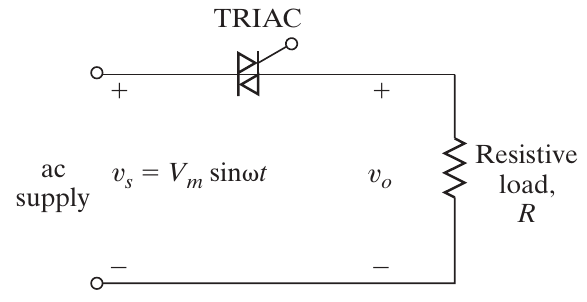
\includegraphics[width=\textwidth,height=3cm,keepaspectratio]{img/ac-ac-conv-dia.png}
		\caption{Circuito}%
		\label{fig:ac-ac-conv-dia} %chktex 24
	\end{subfigure}%
	\begin{subfigure}[b]{0.5\columnwidth}
		\centering
		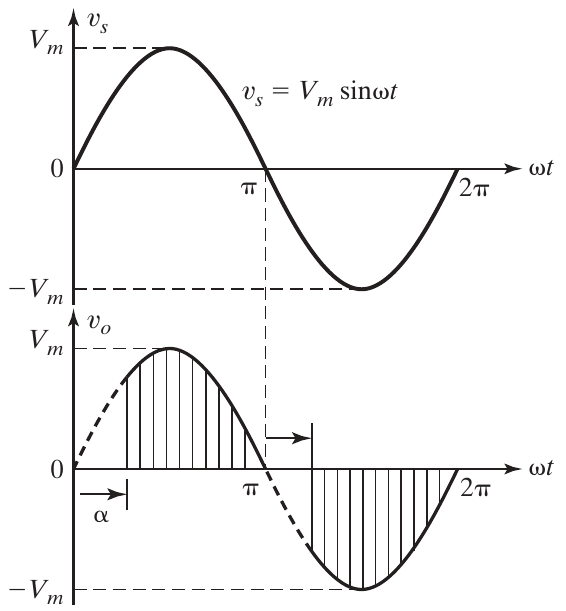
\includegraphics[width=\textwidth,height=5cm,keepaspectratio]{img/ac-ac-conv-wave.png}
		\caption{Señal voltaica}%
		\label{fig:ac-ac-conv-wave} %chktex 24
	\end{subfigure}
	\caption[Convertidor AC-AC]{Convertidor AC-AC de una fase.\footnotemark{}}%
	\label{fig:ac-ac-conv} % chktex 24
\end{figure}
\footnotetext{Fuente de la imagen: \Citet[pp.~33]{Rashid2006}.}

Nótese que los ángulos de defasamiento de voltaje $\theta_v$ y corriente $\theta_i$ han desaparecido.
Esto se debe a que en un circuito de AC de una sola fase $\theta_v = 0$ por ser la única fase y por ende la referencia.
Además, en un circuito puramente resistivo las señales de voltaje y corriente están acopladas, por lo que $\theta_i = \theta_v$ tal como se muestra en la \Cref{fig:ac-v-i}.

\begin{figure}[H]
% \begin{wrapfigure}{r}{0.3\columnwidth}
	\centering
	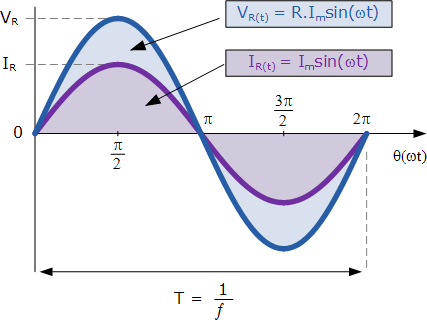
\includegraphics{img/ac-v-i.png}
	\caption[Voltaje y corriente en un circuito resistivo monofase]%
	{Voltaje y corriente en un circuito resistivo monofase.\footnotemark{}}%
	\label{fig:ac-v-i}
	\footnotetext{Fuente de imagen: \url{https://www.electronics-tutorials.ws/accircuits/ac-resistance.html}}
% \end{wrapfigure}
\end{figure}

En la mayoría de los casos lo que interesa no es el cálculo de la potencia neta, sino controlar el factor de potencia, el decir, el porcentaje de la potencia máxima que la carga está entregando.
Al estar sincronizadas la corriente y el voltaje por ser un circuito resistivo y no existir más que una fase, el cálculo de la potencia se simplifica y se convierte en el cociente del voltaje promedio aplicado a la carga respecto al voltaje RMS de la línea.
Es decir

\begin{align}
	P_f = \frac{V_o}{V_{RMS}}
	\label{eq:pf}
\end{align}

\noindent y dado que $V_{RMS}$ es fijo, lo que interesa calcular es el voltaje aplicado a la carga $V_o$ que se calcula como~\Citep[579--583]{Rashid2006}:%
\footnote{El valor medio o efectivo de cualquier función $f(\omega t)$ con periodo de $2\pi rad$ está determinado por
	$F = \sqrt{
		\frac{1}{2\pi}
		\int^{2\pi}_0
		f^2\left(\omega t\right) d\omega t
	}$
}

\begin{align}
	V^2_o = &
		\frac{2}{2\pi}
		\int^\pi_\alpha
		2V^2_{RMS}\sin^2\left(\omega t\right)
		d\left(\omega t\right)
		\\
	= &
		\frac{4V^2_{RMS}}{4\pi}
		\int^\pi_\alpha
		\big(1-\cos\left(2\omega t\right)\big)
		d\left(\omega t\right)
		\\
	= &
		\frac{V^2_{RMS}}{\pi}
		\left(
			\pi-\alpha + \frac{\sin\left(2\alpha\right)}{2}
		\right)
\end{align}

\noindent Por lo tanto

\begin{align}
	V_o = &
		{\left[
			\frac{V^2_{RMS}}{\pi}
			\left(
				\pi-\alpha + \frac{\sin\left(2\alpha\right)}{2}
			\right)
		\right]}^\frac{1}{2}
		\\
	=&
		V_{RMS}\sqrt{
		\frac{1}{\pi}
		\left(
			\pi-\alpha + \frac{\sin\left(2\alpha\right)}{2}
		\right)
		}
	\label{eq:po}
\end{align}

Ahora, supóngase que se desea modular la potencia de un foco incandescente de $60W$ conectado a una línea estándar de $V_{RMS}=120V$, 60Hz.
Como $P=\frac{V^2}{R}$ se puede calcular tanto la resistencia del foco como la corriente a fin de elegir el TRIAC adecuado:

\begin{align*}
	R =& \frac{V^2}{P} \\
	=&
		\frac{{\left(120V\right)}^2}{60W} \\
	=&
		\frac{14400V^2}{60W} \\
	=& 240\Omega
\end{align*}

\noindent y como $I=\frac{V}{R}$
\begin{align*}
	I_{RMS} & = \frac{120V}{240\Omega} = 0.5A\\
	I_{m} & = \sqrt{2} \times I_{RMS} =\sqrt{2} \times 0.5A\\
	      & = 0.7A
\end{align*}

\cleardoublepage
Ahora bien, si se usa un ángulo de disparo en el TRIAC de $\alpha = \frac{\pi}{2}$ la potencia de el foco con base en las \Cref{eq:pf,eq:po} será:

\begin{align*}
	P_f &= \frac{V_o}{V_{RMS}} \\
	&= \frac{\cancel{V_{RMS}}{~\left[
			\frac{1}{\pi}
			\left(
				\pi-\alpha + \frac{\sin\left(2\alpha\right)}{2}
			\right)
			\right]}^\frac{1}{2}
		}{\cancel{V_{RMS}}}
	\\
	&=
		{~\left[
			\frac{1}{\pi}
			\left(
				\cancelto{\frac{\pi}{2}}{\pi-\frac{\pi}{2}} +
				\frac{\sin\left(\frac{\cancel{2}\pi}{\cancel{2}}\right)}{2}
			\right)
		\right]}^\frac{1}{2}
	\\
	&=
		{\left[
			\frac{1}{\pi}
			\left(
				\frac{\pi}{2} +
				\cancelto{0}{\frac{\sin\left(\pi\right)}{2}}
			~~~\right)
		\right]}^\frac{1}{2}
	\\
	&=
		{\left(
			\frac{1}{\cancel{\pi}}
			\cdot
			\frac{\cancel{\pi}}{2}
		\right)}^\frac{1}{2}
	\\
	&= \sqrt{\frac{1}{2}}\\
	&= 0.707 \\
	&= 70.7\%
\end{align*}

De este desarrollo se concluye, además, que el factor de potencia no depende de los valores de voltaje, sino sólo del ángulo de disparo del TRIAC $\alpha$.

Como $\alpha = \omega t$, para conocer el tiempo de disparo $\tau$ basta con sustituir $t=\tau$ y despejar.
Así:

\begin{align*}
	\tau =& \frac{\alpha}{\omega} \\
	=&
		\frac{\alpha}{2 \pi f} \\
	=&
		\frac{\frac{\pi}{2}}{2 \pi f}\bigg\rvert_{f=60\text{Hz}}
		\\
	=&
		\frac{1}{4 \times 60\text{Hz}} =
		\frac{1}{240\text{Hz}}
		\\
	=& 0.00416\bar{6}\text{s} \\
	\approx& 4.2\text{ms}
\end{align*}

Un problema importante a considerar es que la ecuación
\(
	P_f = {~\left[
		\frac{1}{\pi}
		\left(
			\pi-\alpha + \frac{\sin\left(2\alpha\right)}{2}
		\right)
	\right]}^\frac{1}{2}
\)
no es biyectiva (tiene una componente periódica senoidal) y por lo tanto no es posible calcular su inversa de forma analítica.
En otras palabras, no es posible obtener una expresión algebraica para calcular $\alpha\left(P_f\right)$, y por tampoco es posible inferir $\tau\left(P_f\right)$.

Existen varias soluciones alterna a este problema.
Por ejemplo, pueden utilizarse varios métodos de aproximación numérica para cada uno de los segmentos de la curva y utilizar el más adecuado para en cada uno de los rangos de interés.
Otros métodos que requieren un número mucho menor de cálculos hacen uso de una tabla de valores discretos (por ejemplo incrementos de 1\% en el factor de potencia) e interpolan linealmente entre estos, dejando el error como una perturbación a corregir por el controlador (véase \Cref{tbl:trigger-time}).

\begin{table}[H]
	\centering
	\captionsetup{justification=centering,margin=2cm}
	\caption{Relación entre factor de potencia y tiempo de disparo de TRIAC\\Tabla para interpolación con incrementos de 5\% y alimentación de AC a 60Hz}%
	\label{tbl:trigger-time}
	\begin{tabular}{c c  c c  c c}
		\toprule
		\textbf{\small Factor de} &
		\textbf{\small Tiempo de} &
		\textbf{\small Factor de} &
		\textbf{\small Tiempo de} &
		\textbf{\small Factor de} &
		\textbf{\small Tiempo de}\\
		\textbf{\small potencia [\%]} &
		\textbf{\small disparo [ms]}  &
		\textbf{\small potencia [\%]} &
		\textbf{\small disparo [ms]}  &
		\textbf{\small potencia [\%]} &
		\textbf{\small disparo [ms]} \\
		\midrule
		100 & 0.000 &  65 & 4.464 &  30 & 6.232 \\
		 95 & 2.060 &  60 & 4.734 &  25 & 6.487 \\
		 90 & 2.696 &  55 & 4.993 &  20 & 6.750 \\
		 85 & 3.157 &  50 & 5.245 &  15 & 7.030 \\
		 80 & 3.538 &  45 & 5.493 &  10 & 7.334 \\
		 75 & 3.874 &  40 & 5.738 &   5 & 7.688 \\
		 70 & 4.179 &  35 & 5.984 &   0 & 8.203 \\
		\bottomrule
	\end{tabular}
\end{table}
